\chapter{Batch Script Transformer}

This tool once had been a least used one due to its limitations. Now with the new transliterating engine, the tool becomes more usable and quite useful for converting a bunch of files. Common users may not see the necessity of this, but for those who deal with text collections, this tool is a kind of magic bullet.

The tool can be launched by menu File > {\faSix \symbol{"F085}} Batch Script Transformer. Here are basic considerations:

\begin{itemize}
\item The input texts can be either in plain text or XML/HTML-like structure, but not JSON.\footnote{The program does not exactly detect the format structure. XML/HTML uses tags to differentiate data from metadata, which is easy to set apart, but not so in JSON. Practically, converting non-Roman texts in JSON to Roman is applicable, but not vice versa. When reading Roman text, the program cannot tell data apart from metadata because both normally use the same character blocks.} XML files of the CST collections are the main target with special treatments. The tool also works fine with texts in HTML.
\item The input script can be auto-detected or manually specified (see {\faSix \symbol{"F560}} menu button).\footnote{Supported input and output scripts so far are Roman (various transliteration methods), Devanāgarī, Khmer, Myanmar, Sinhala, and Thai. Other potential scripts can be suggested to the author, who naturally prefers `just enough' over `all-embracing'.}
\item The encoding of input files has to be set properly, either UTF-8 or UTF-16 (other formats are unsupported). We should see UTF-8 most of the time, but Tipitaka.org's CST XMLs are in UTF-16, like most files produced in Windows. The encoding has to be set before adding files, otherwise the files cannot be read properly.
\end{itemize}

\boxnote{If the script of source files cannot be auto-detected, probably the file encoding is wrongly set. Try switching to another encoding (UTF-16 or UTF-8), and adding files again.}

The basic operations of the tool are as follows: 

\begin{compactenum}
\item Select file encoding, either UTF-8 (default) or UTF-16 (mainly used with CST Devanāgarī)
\item Add source files
\item Select input script or left auto-detected
\item Select output script (only one per session)
\item Select output directory or use the source's directory
\item Press {\faSix \symbol{"F085}} Convert
\item When green check marks are seen, the conversion is successful, and the output files are created with new names prefixed by output script
\end{compactenum}

Figure \ref{fig:batch-transformer} shows an example of a conversion of CST Devanāgarī files to Roman.

\begin{figure}[!hbt]
\centering
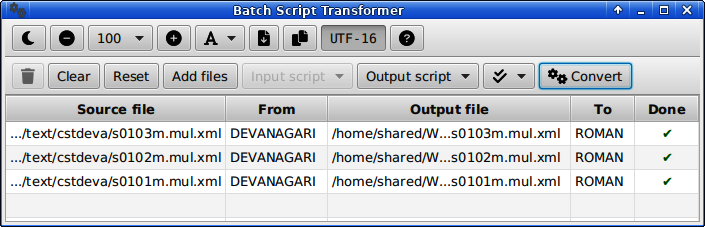
\includegraphics[width=0.9\linewidth]{images/batch-transformer.png}\\
\caption{Basic use of Batch Script Transformer}
\label{fig:batch-transformer}
\end{figure}

When converting any scripts to Roman, you have to pay more attention to the transliteration methods, as shown in Figure \ref{fig:batch-transformer-options} (see also Section \ref{sect:roman-translit} on page \pageref{sect:roman-translit}).

When converting a Roman text, you have to be aware whether the source text is Sanskrit or not. If so, the option of \emph{Roman as Sanskrit} has to be enabled, otherwise the conversion may be incorrect. You also have an option to include or exclude Roman numbers in conversion.

\begin{figure}[!hbt]
\centering
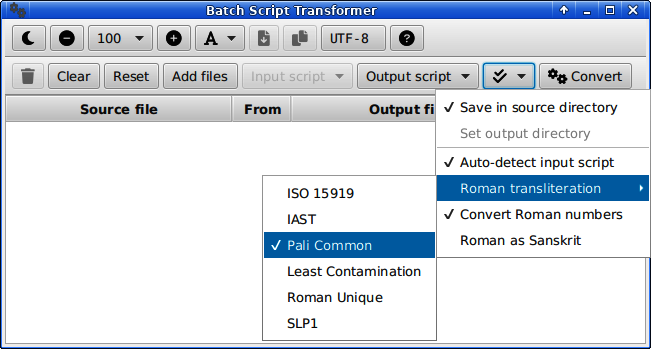
\includegraphics[width=0.9\linewidth]{images/batch-transformer-options.png}\\
\caption{Options for Roman transliteration}
\label{fig:batch-transformer-options}
\end{figure}

